% Provenance (never printed): cycle 4 SVT, "La planete Terre, l'environnement":
% glaciers and their landforms, the cryosphere, the glaciations told; see
% sources/book1/PROVENANCE.md. Book 1, grade 8, chapter 5.
% Vocabulary guard: owns glacier; ice sheet + ice shelf + iceberg (one
% definition); sea ice; permafrost; U-shaped valley + moraine (one
% definition); ice age. "Glacial period", "interglacial" and "glacial cycle"
% belong to Book 2 g12 past-climates: here "the ice ages and the warmer times
% between them", in prose. Albedo belongs to Book 2 g10: here "reflects".
% Buoyancy and water expanding as it freezes are physics: recalled in prose.
\chapter{Es di Bumi}\label{ch:g8:ice-on-earth}

Kedua foto di bawah diambil dari tempat yang sama, di sebuah laguna di
Alaska, dengan selang waktu 26 tahun. Pada tahun 1990, lidah es yang lebar
turun menyusuri \omterm{def:g1:landscapes-around-us:landform}{lembah} sampai ke air. Pada tahun 2016, es itu sudah mundur
ke hulu \omterm{def:g1:landscapes-around-us:landform}{lembah} dan menjadi lebih sempit; pepohonan dan \omterm{def:g3:stones-pebbles-sand:rock}{batuan} gundul
mengisi ruang yang ditinggalkannya. Citra satelit menunjukkan bahwa antara
tahun 1984 dan 2021, ujung depan \omterm{def:g8:ice-on-earth:glacier}{gletser} ini, \omterm{def:g8:ice-on-earth:glacier}{Gletser} Pedersen, mundur
sekitar \qty{3.2}{km}.
% ledger: commons:pedersen, uw:pedersen

\begin{omfigure}
\begin{minipage}[t]{0.49\linewidth}\centering
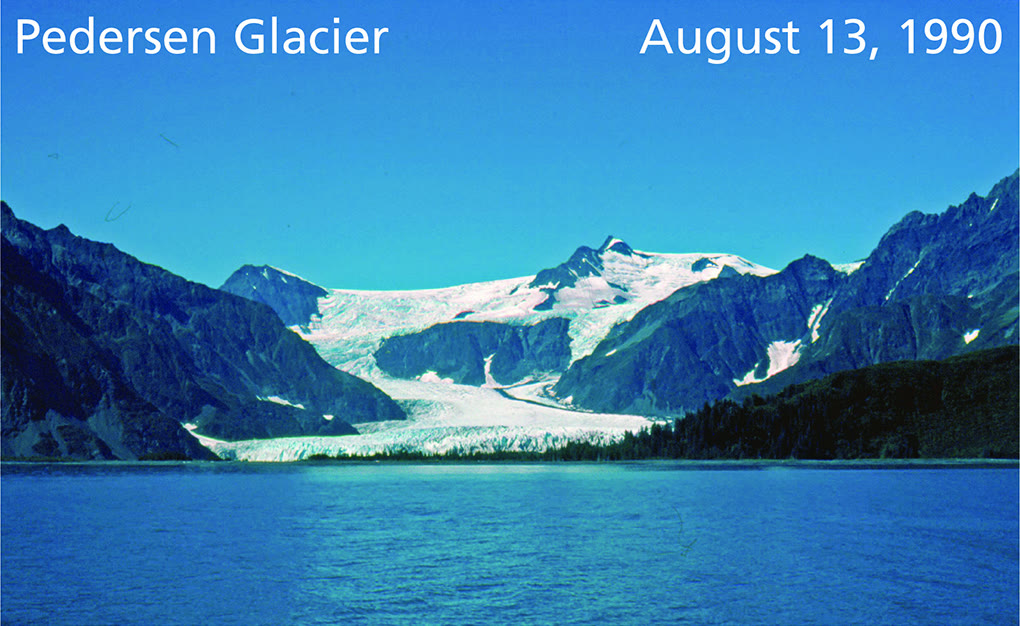
\includegraphics[width=\linewidth]{images/book1/g8-pedersen-1990.jpg}
\end{minipage}\hfill
\begin{minipage}[t]{0.49\linewidth}\centering
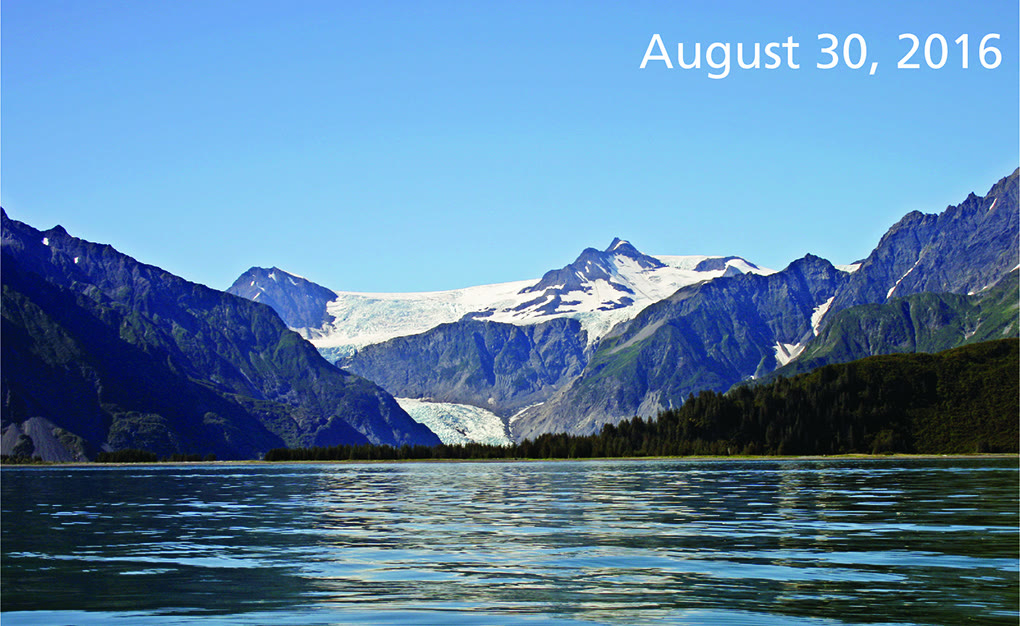
\includegraphics[width=\linewidth]{images/book1/g8-pedersen-2016.jpg}
\end{minipage}

\smallskip
{\small \omterm{def:g8:ice-on-earth:glacier}{Gletser} Pedersen, Taman Nasional Kenai Fjords, Alaska, dilihat dari
tempat yang sama pada 13~Agustus 1990 (kiri, foto oleh M.~Tetreau) dan
pada 30~Agustus 2016 (kanan, foto oleh D.~Kurtz). U.S. National Park
Service, domain publik (melalui Wikimedia Commons).}
% ledger: commons:pedersen
\label{fig:g8:ice-on-earth:pedersen}
\end{omfigure}

Sekarang es menutupi sekitar sepersepuluh daratan di Bumi. Es itu terdapat
di \omterm{def:g1:landscapes-around-us:landform}{lembah-lembah} \omterm{def:g4:world-physical-map:range}{pegunungan}, dalam dua lapisan raksasa di atas Antarktika
dan Greenland, di \omterm{def:g2:water-on-earth:ocean}{laut-laut} \omterm{def:g3:continents-and-oceans:poles}{kutub}, dan, tersembunyi, di dalam tanah yang
membeku di ujung utara. Bab ini membahas masing-masing secara bergiliran,
cara es membentuk daratan, dan masa-masa ketika es menutupi jauh lebih
banyak bagian Bumi daripada sekarang.
% ledger: nsidc:ice-cover

\begin{recall}
\omterm{def:g4:clouds-rain-snow:precipitation}{Salju} adalah salah satu jenis \omterm{def:g4:clouds-rain-snow:precipitation}{presipitasi}: kristal-kristal es yang tumbuh
di dalam \omterm{def:g4:clouds-rain-snow:cloud}{awan} dan jatuh tanpa mencair (\cref{ch:g4:clouds-rain-snow}). Air
yang mengalir mengikis daratan, membawa pecahan-pecahannya pergi, dan
mengendapkannya lebih jauh di hilir; \omterm{def:g1:landscapes-around-us:water}{sungai} mengukir \omterm{def:g1:landscapes-around-us:landform}{lembah}
(\cref{ch:g5:water-shapes-the-land}). Ketika air \omterm{def:g2:water-on-earth:ocean}{laut} membeku, garamnya
tertinggal di air di sekitar es (\cref{ch:g8:the-oceans}). Dalam fisika,
kamu belajar bahwa air memuai ketika membeku, sehingga es kurang rapat
daripada air cair, dan bahwa benda yang lebih ringan daripada air yang
didesaknya akan mengapung.
\end{recall}

\section{Gletser}

Tinggi di \omterm{def:g4:world-physical-map:range}{pegunungan}, \omterm{def:g4:clouds-rain-snow:precipitation}{salju} yang turun pada musim dingin lebih banyak
daripada yang mencair pada musim panas. Tahun demi tahun, \omterm{def:g4:clouds-rain-snow:precipitation}{salju} baru
mengubur \omterm{def:g4:clouds-rain-snow:precipitation}{salju} lama dan menekannya. Kristal-kristalnya saling memadat,
udara di antaranya terperas keluar, dan setelah sekitar satu tahun \omterm{def:g4:clouds-rain-snow:precipitation}{salju}
itu menjadi \emph{firn}, bahan berbutir yang berada di antara \omterm{def:g4:clouds-rain-snow:precipitation}{salju} dan
es. Terkubur makin dalam, firn berubah menjadi es yang keras dan padat;
pada kebanyakan \omterm{def:g8:ice-on-earth:glacier}{gletser}, proses ini memakan waktu lebih dari seratus
tahun.
% ledger: nsidc:firn

\begin{definition}[Gletser]\label{def:g8:ice-on-earth:glacier}
Yang disebut \emph{gletser}\index{gletser} adalah massa es, yang terbentuk
dari \omterm{def:g4:clouds-rain-snow:precipitation}{salju} yang menumpuk selama bertahun-tahun, yang bergerak perlahan
menuruni lereng di atas daratan karena beratnya sendiri.
\end{definition}
% ledger: nsidc:glacier-def

\omterm{def:g8:ice-on-earth:glacier}{Gletser} mempunyai dua bagian. Di bagian atasnya, \emph{daerah akumulasi},
\omterm{def:g4:clouds-rain-snow:precipitation}{salju} yang turun setiap tahun lebih banyak daripada yang mencair: \omterm{def:g8:ice-on-earth:glacier}{gletser}
bertambah es. Di bagian bawahnya, \emph{daerah ablasi}, es yang mencair
setiap tahun lebih banyak daripada \omterm{def:g4:clouds-rain-snow:precipitation}{salju} yang turun: \omterm{def:g8:ice-on-earth:glacier}{gletser} kehilangan es.
Es yang bertambah di atas terus mengalir turun untuk menggantikan es yang
hilang di bawah. Jika keduanya seimbang, ujung depan \omterm{def:g8:ice-on-earth:glacier}{gletser}, yaitu
\emph{moncong}nya, tetap berada di tempat yang sama.
% ledger: nsidc:glacier-zones

\begin{omfigure}
\begin{tikzpicture}[font=\footnotesize, >={Stealth[length=2mm]}, xscale=1.08]
  % bedrock
  \fill[black!13] (0,4.6) -- (2,3.9) -- (4,3.0) -- (6,2.0) -- (8,1.1)
    -- (10,0.45) -- (11,0.3) -- (13,0.15) -- (13,-0.5) -- (0,-0.5) -- cycle;
  % the ice body, two zones
  \begin{scope}
    \clip (0,5.5) -- (2,4.9) -- (4,4.0) -- (6,2.9) -- (8,1.8) -- (9.4,0.95)
      -- (10,0.45) -- (8,1.1) -- (6,2.0) -- (4,3.0) -- (2,3.9) -- (0,4.6) -- cycle;
    \fill[omIce] (0,-1) rectangle (5,6);
    \fill[omSea!85] (5,-1) rectangle (11,6);
  \end{scope}
  \draw[black!60] (0,5.5) -- (2,4.9) -- (4,4.0) -- (6,2.9) -- (8,1.8)
    -- (9.4,0.95) -- (10,0.45);
  \draw[black!70, line width=0.6pt] (0,4.6) -- (2,3.9) -- (4,3.0) -- (6,2.0)
    -- (8,1.1) -- (10,0.45) -- (11,0.3) -- (13,0.15);
  % snowline
  \draw[dashed, black!70] (5,2.5) -- (5,4.15);
  \node[anchor=south] at (5,4.15) {salju turun = salju mencair};
  % snowflakes and melting
  \foreach \x/\y in {0.5/6.1, 1.3/5.8, 2.1/5.5, 2.9/5.1, 3.7/4.8, 0.9/6.6, 1.7/6.3, 2.5/6.0, 3.3/5.6, 4.1/5.2}
    \node[omCold] at (\x,\y) {$\ast$};
  \foreach \x/\y in {6.4/2.8, 7.2/2.35, 8.0/1.9}
    \draw[omWarm, decorate, decoration={snake, amplitude=0.6mm, segment length=2mm}] (\x,\y) -- ++(0,0.6);
  % flow arrows inside the ice
  \draw[->, omDef, line width=0.9pt] (1.0,4.72) -- (2.2,4.30);
  \draw[->, omDef, line width=0.9pt] (3.0,3.95) -- (4.2,3.41);
  \draw[->, omDef, line width=0.9pt] (5.2,2.88) -- (6.4,2.28);
  \draw[->, omDef, line width=0.9pt] (7.2,1.84) -- (8.3,1.35);
  % moraine and meltwater
  \fill[omLithCongl] (10.15,0.42) .. controls (10.5,0.95) and (10.9,0.95) .. (11.2,0.29) -- cycle;
  \draw[omSea!60!black, line width=1.6pt] (10.05,0.38) .. controls (10.6,0.22) and (11.4,0.12) .. (12.9,0.08);
  % labels
  \node[align=center] at (1.9,7.15) {daerah akumulasi:\\ salju menumpuk, gletser bertambah es};
  \node[align=center] at (10.0,3.3) {daerah ablasi:\\ es mencair, gletser kehilangan es};
  \node[align=left, anchor=west, omDef] at (4.4,1.3) {es mengalir\\ menuruni lereng};
  \draw[black!60] (10.0,0.5) -- (9.6,-0.1) node[below] {moncong};
  \draw[black!60] (10.7,0.85) -- (11.3,1.4) node[above] {morena};
  \node[anchor=north east] at (12.9,0.0) {aliran air lelehan};
  \node at (2.2,2.6) {batuan dasar};
\end{tikzpicture}

{\small \omterm{def:g8:ice-on-earth:glacier}{Gletser} \omterm{def:g1:landscapes-around-us:landform}{lembah} dilihat dalam penampang memanjang (sketsa, tidak
berskala). Di atas garis putus-putus, \omterm{def:g4:clouds-rain-snow:precipitation}{salju} menumpuk lebih cepat daripada
mencairnya; di bawahnya, es mencair lebih cepat daripada turunnya \omterm{def:g4:clouds-rain-snow:precipitation}{salju}.
Es mengalir turun dari bagian yang satu ke bagian yang lain.}
\label{fig:g8:ice-on-earth:long-section}
\end{omfigure}

Bagaimana es yang padat dapat mengalir? Di bawah berat es di atasnya, es
yang berada jauh di dalam \omterm{def:g8:ice-on-earth:glacier}{gletser} perlahan-lahan berubah bentuk, seperti
lapisan tebal madu dingin yang meluber. \omterm{def:g8:ice-on-earth:glacier}{Gletser} juga meluncur di atas
\omterm{def:g3:stones-pebbles-sand:rock}{batuan} di bawahnya, di atas selapis tipis air atau \omterm{def:g3:stones-pebbles-sand:sand}{lumpur} basah. Bagian
bawah \omterm{def:g8:ice-on-earth:glacier}{gletser}, yang bergesekan dengan \omterm{def:g3:stones-pebbles-sand:rock}{batuan}, bergerak lebih lambat
daripada bagian atasnya. Kebanyakan \omterm{def:g8:ice-on-earth:glacier}{gletser} bergerak lambat dan tetap;
beberapa tiba-tiba \emph{melonjak}. Pada tahun 1986, \omterm{def:g8:ice-on-earth:glacier}{Gletser} Hubbard di
Alaska melonjak maju sekitar \qty{10}{m} sehari, dan lonjakan tercepat
yang pernah tercatat, \omterm{def:g8:ice-on-earth:glacier}{Gletser} Kutiah di Pakistan pada tahun 1953,
rata-rata sekitar \qty{112}{m} sehari selama tiga bulan.
% ledger: nsidc:glacier-flow, nsidc:surges

Ketika \omterm{def:g8:ice-on-earth:glacier}{gletser} kehilangan lebih banyak es di bawah daripada yang
diperolehnya di atas, moncongnya bergerak mundur ke hulu \omterm{def:g1:landscapes-around-us:landform}{lembah}: \omterm{def:g8:ice-on-earth:glacier}{gletser}
itu \emph{menyusut}. \omterm{def:g8:ice-on-earth:glacier}{Gletser} yang menyusut tetap mengalir menuruni lereng,
seperti ban berjalan; hanya saja ia mencair lebih cepat daripada
mengalirnya. \omterm{def:g8:ice-on-earth:glacier}{Gletser} Muir, di Alaska, mengisi seluruh \omterm{def:g1:landscapes-around-us:landform}{lembahnya} sampai ke
\omterm{def:g2:water-on-earth:ocean}{laut} pada tahun 1941. Pada tahun 2004, moncongnya sudah mundur
\qty{12}{km}, dan permukaan esnya sudah turun lebih dari \qty{800}{m}.
% ledger: nsidc:glacier-flow, nsidc:muir

\section{Bagaimana es membentuk lembah}

\omterm{def:g8:ice-on-earth:glacier}{Gletser} adalah alat \omterm{def:g5:water-shapes-the-land:erosion}{erosi} yang sangat kuat. Esnya membeku melekat pada
bongkah-bongkah \omterm{def:g3:stones-pebbles-sand:rock}{batuan} yang lepas lalu mencabutnya; batu-batu yang
membeku di dasarnya menggerus \omterm{def:g3:stones-pebbles-sand:rock}{batuan} di bawahnya seperti amplas. \omterm{def:g8:ice-on-earth:glacier}{Gletser}
membawa semua \omterm{def:g3:stones-pebbles-sand:rock}{batuan} ini, dari debu halus sampai bongkah raksasa,
menuruni \omterm{def:g1:landscapes-around-us:landform}{lembah} seperti ban berjalan, lalu menjatuhkannya di tempat esnya
mencair.
% ledger: nps:u-valley

\begin{omfigure}
\begin{tikzpicture}[font=\footnotesize, >={Stealth[length=2mm]}]
  % V-shaped valley
  \fill[black!13] (0,3) -- (2.1,0.35) -- (2.5,0.35) -- (4.6,3) -- (4.6,-0.4) -- (0,-0.4) -- cycle;
  \draw[black!70, line width=0.6pt] (0,3) -- (2.1,0.35) -- (2.5,0.35) -- (4.6,3);
  \fill[omSea] (2.1,0.35) -- (2.5,0.35) -- (2.42,0.2) -- (2.18,0.2) -- cycle;
  \node[align=center] at (2.3,-0.85) {sungai mengukir lembah\\ berbentuk V yang sempit};
  % arrow
  \draw[->, line width=1pt] (5.0,1.5) -- (6.2,1.5) node[midway, above, align=center] {gletser\\ mengisinya};
  % U-shaped valley
  \begin{scope}[xshift=6.6cm]
    \fill[black!13] (0,3) .. controls (0.6,1.0) and (0.9,0.25) .. (1.6,0.2)
      -- (3.0,0.2) .. controls (3.7,0.25) and (4.0,1.0) .. (4.6,3) -- (4.6,-0.4) -- (0,-0.4) -- cycle;
    \draw[black!70, line width=0.6pt] (0,3) .. controls (0.6,1.0) and (0.9,0.25) .. (1.6,0.2)
      -- (3.0,0.2) .. controls (3.7,0.25) and (4.0,1.0) .. (4.6,3);
    \draw[dashed, black!40] (0,3) -- (2.1,0.35) -- (2.5,0.35) -- (4.6,3);
    \draw[omCold, line width=0.9pt] (0.37,2.2) -- (4.23,2.2);
    \node[omCold, anchor=south, font=\scriptsize] at (2.3,2.2) {permukaan es, dahulu kala};
    \fill[omLithCongl] (0.75,0.95) .. controls (0.95,1.2) and (1.1,1.1) .. (1.2,0.6) -- cycle;
    \fill[omLithCongl] (3.85,0.95) .. controls (3.65,1.2) and (3.5,1.1) .. (3.4,0.6) -- cycle;
    \node[align=center] at (2.3,-0.85) {setelah es lenyap: lembah lebar\\ berbentuk U, dinding curam};
    \draw[black!60] (3.65,0.95) -- (4.85,0.6) node[right, align=left] {morena\\ lateral};
    \node[font=\scriptsize, black!55, align=center] at (2.3,1.6) {(V lama, putus-putus)};
  \end{scope}
\end{tikzpicture}

{\small \omterm{def:g1:landscapes-around-us:landform}{Lembah} \omterm{def:g1:landscapes-around-us:landform}{gunung} yang sama dalam penampang melintang, sebelum dan
sesudah dilalui \omterm{def:g8:ice-on-earth:glacier}{gletser} (sketsa). Es menggerus \omterm{def:g1:landscapes-around-us:landform}{lembah} \omterm{def:g1:landscapes-around-us:water}{sungai} yang sempit
menjadi palung yang lebar dengan dasar yang luas dan dinding yang curam,
dan meninggalkan pematang puing \omterm{def:g3:stones-pebbles-sand:rock}{batuan} di sepanjang tepinya.}
\label{fig:g8:ice-on-earth:v-and-u}
\end{omfigure}

\begin{definition}[Lembah berbentuk U dan morena]\label{def:g8:ice-on-earth:glacial-landforms}
Yang disebut \emph{lembah berbentuk U}\index{lembah berbentuk U} adalah
\omterm{def:g1:landscapes-around-us:landform}{lembah} dengan dasar yang lebar dan datar serta dinding yang curam, yang
diukir oleh \omterm{def:g8:ice-on-earth:glacier}{gletser} yang melebarkan dan mendalamkan \omterm{def:g1:landscapes-around-us:landform}{lembah} \omterm{def:g1:landscapes-around-us:water}{sungai}
berbentuk V yang sempit. Yang disebut \emph{morena}\index{morena} adalah
pematang puing \omterm{def:g3:stones-pebbles-sand:rock}{batuan}, dari debu sampai bongkah, yang ditinggalkan oleh
\omterm{def:g8:ice-on-earth:glacier}{gletser}: \emph{morena lateral} di sepanjang sisinya, \emph{morena
terminal} di ujungnya.
\end{definition}
% ledger: usgs:erratic, nps:u-valley, nps:moraines

\omterm{def:g8:ice-on-earth:glacial-landforms}{Morena} adalah petunjuk yang berguna. \omterm{def:g8:ice-on-earth:glacial-landforms}{Morena} terminal yang jauh di hilir
\omterm{def:g1:landscapes-around-us:landform}{lembah}, tanpa es sedikit pun di dekatnya, menunjukkan seberapa jauh
\omterm{def:g8:ice-on-earth:glacier}{gletser} itu dahulu mencapai; \omterm{def:g8:ice-on-earth:glacial-landforms}{morena} lateral yang tinggi di sisi \omterm{def:g1:landscapes-around-us:landform}{lembah}
menunjukkan seberapa tebal es itu dahulu. Bongkah besar yang tergeletak
sendirian di sebuah ladang, terbuat dari \omterm{def:g3:stones-pebbles-sand:rock}{batuan} yang tidak ditemukan di
mana pun di sekitarnya, adalah petunjuk lain: itulah \emph{batu eratik},
\omterm{def:g3:stones-pebbles-sand:rock}{batuan} yang dibawa \omterm{def:g8:ice-on-earth:glacier}{gletser} jauh dari tempat asalnya dan ditinggalkan
ketika esnya mencair. Ukuran batu eratik beragam, dari \omterm{def:g3:stones-pebbles-sand:pebble}{kerikil} sampai
bongkah yang lebih besar daripada rumah.
% ledger: nps:moraines, usgs:erratic

\begin{inthefield}[Membaca lembah yang dibentuk es]
Saat berjalan-jalan di \omterm{def:g4:world-physical-map:range}{pegunungan}, atau pada foto sebuah \omterm{def:g1:landscapes-around-us:landform}{lembah} \omterm{def:g1:landscapes-around-us:landform}{gunung},
perhatikan bentuk \omterm{def:g1:landscapes-around-us:landform}{lembah} itu dalam penampang melintang: V yang sempit,
atau U yang lebar dengan dinding yang curam? Carilah di dasar \omterm{def:g1:landscapes-around-us:landform}{lembah}
pematang-pematang panjang dari batu dan tanah yang campur aduk, yang
membentang di sepanjang sisinya atau melintanginya: mungkin itu \omterm{def:g8:ice-on-earth:glacial-landforms}{morena}.
Carilah bongkah-bongkah besar yang tidak sesuai dengan \omterm{def:g3:stones-pebbles-sand:rock}{batuan} di
sekitarnya, dan permukaan \omterm{def:g3:stones-pebbles-sand:rock}{batuan} halus yang tergores garis-garis panjang
yang sejajar. Tetaplah di jalan setapak, jauhi tepi lereng yang curam dan
es itu sendiri, dan gambarlah apa yang kamu lihat di buku catatanmu.
\end{inthefield}

\section{Lapisan es, paparan es, dan gunung es}

Massa es terbesar di Bumi tidak berada di \omterm{def:g1:landscapes-around-us:landform}{lembah} \omterm{def:g4:world-physical-map:range}{pegunungan}: massa es itu
menutupi seluruh daratan. \omterm{def:g8:ice-on-earth:ice-sheet}{Lapisan es} Antarktika membentang di atas hampir
\num{14}~juta~\unit{km^2} dan tebalnya hampir \qty{4.9}{km} di bagian
yang paling tebal. \omterm{def:g8:ice-on-earth:ice-sheet}{Lapisan es} Greenland menutupi sekitar
\num{1.7}~juta~\unit{km^2}, empat perlima pulau itu, dan tebalnya lebih
dari \qty{3}{km}. Bersama-sama, keduanya menyimpan lebih dari 99~\% es di
daratan, dan lebih dari dua pertiga seluruh \omterm{def:g2:water-on-earth:salt-fresh}{air tawar} di Bumi.
% ledger: nsidc:ice-sheets

\begin{definition}[Lapisan es, paparan es, dan gunung es]\label{def:g8:ice-on-earth:ice-sheet}
Yang disebut \emph{lapisan es}\index{lapisan es} adalah massa es yang
menutupi daratan seluas lebih dari \qty{50000}{km^2}, seperti kubah
raksasa yang meluas ke segala arah. Di tempat es yang mengalir dari
daratan mencapai \omterm{def:g2:water-on-earth:ocean}{laut} dan terus mengapung di atasnya, sambil masih
tersambung dengan es di belakangnya, terbentuklah \emph{paparan
es}\index{paparan es}. Yang disebut \emph{gunung es}\index{gunung es}
adalah bongkah es yang besar, lebih dari \qty{5}{m} lebarnya, yang patah
dari \omterm{def:g8:ice-on-earth:glacier}{gletser} atau paparan es dan mengapung di \omterm{def:g2:water-on-earth:ocean}{laut}.
\end{definition}
% ledger: nsidc:ice-sheets, nsidc:ice-shelves, nsidc:iceberg

\begin{omfigure}
\begin{minipage}[c]{0.5\linewidth}\centering
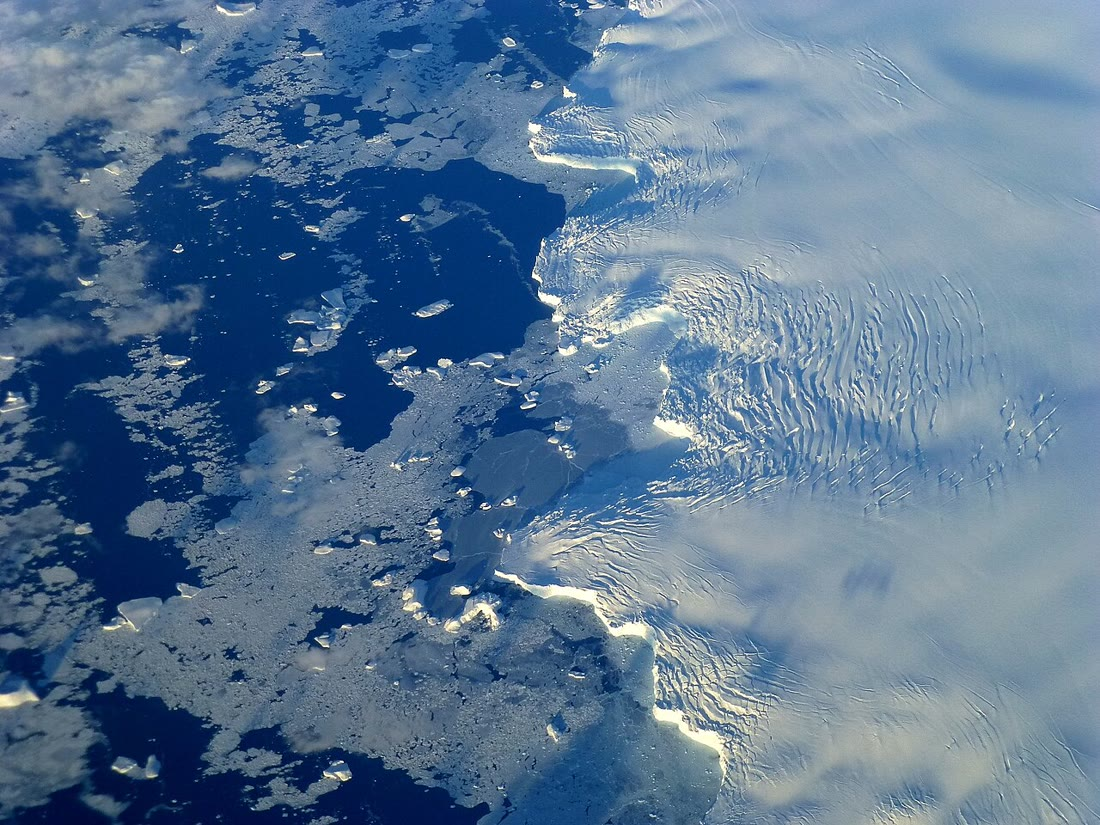
\includegraphics[width=\linewidth]{images/book1/g8-ice-shelf-edge.jpg}
\end{minipage}\hfill
\begin{minipage}[c]{0.46\linewidth}\raggedright
{\small Tepi sebuah \omterm{def:g8:ice-on-earth:ice-sheet}{paparan es} di dekat Pulau Adelaide, di lepas
Semenanjung Antarktika, dilihat dari pesawat terbang pada 28~Oktober 2012.
Es putih yang tebal dan berkerut di kanan adalah \omterm{def:g8:ice-on-earth:ice-sheet}{paparan es}; di kiri,
pecahan-pecahan \omterm{def:g8:ice-on-earth:sea-ice}{es laut} yang lebih tipis mengapung di air yang gelap.
NASA, Operasi IceBridge (domain publik, melalui Wikimedia Commons).}
\end{minipage}
% ledger: commons:ice-shelf
\label{fig:g8:ice-on-earth:ice-shelf}
\end{omfigure}

Air yang terkunci di dalam \omterm{def:g8:ice-on-earth:ice-sheet}{lapisan es} berasal dari \omterm{def:g2:water-on-earth:ocean}{samudra}: air itu
menguap, jatuh sebagai \omterm{def:g4:clouds-rain-snow:precipitation}{salju}, dan menumpuk di daratan. Jika seluruh es
Greenland mencair, \omterm{def:g4:world-physical-map:altitude}{permukaan laut} akan naik sekitar \qty{7.4}{m}; jika
seluruh es Antarktika mencair, sekitar \qty{58}{m}. Semua \omterm{def:g8:ice-on-earth:glacier}{gletser} \omterm{def:g1:landscapes-around-us:landform}{gunung} di
dunia, yang jumlahnya lebih dari \num{200000}, hanya akan menambahkan
kurang dari setengah meter.
% ledger: nsidc:ice-sheets, nsidc:ice-cover

\begin{omfigure}
\begin{tikzpicture}
\begin{axis}[omrecord, xbar, width=10.5cm, height=3.6cm, xmin=0, xmax=68,
  bar width=9pt, ytick=data, symbolic y coords={gletser,Greenland,Antarktika},
  yticklabels={semua gletser gunung, lapisan es Greenland, lapisan es Antarktika},
  xlabel={kenaikan laut jika semuanya mencair (m)}, enlarge y limits=0.3,
  nodes near coords, nodes near coords style={font=\footnotesize, anchor=west, fill=white, inner sep=1.5pt},
  ymajorgrids=false]
  \addplot[fill=omIce!80!black, draw=black!60] coordinates {(0.5,gletser) (7.4,Greenland) (58,Antarktika)};
\end{axis}
\end{tikzpicture}

{\small Seberapa tinggi \omterm{def:g2:water-on-earth:ocean}{laut} akan naik jika setiap jenis es daratan
mencair seluruhnya (nilai dari National Snow and Ice Data Center; nilai
untuk \omterm{def:g8:ice-on-earth:glacier}{gletser} adalah batas atas, ``sedikit di bawah setengah meter'').}
% ledger: nsidc:ice-sheets, nsidc:ice-cover
\label{fig:g8:ice-on-earth:sea-level-bars}
\end{omfigure}

Es yang mengapung lain halnya. \omterm{def:g8:ice-on-earth:ice-sheet}{Paparan es} atau \omterm{def:g8:ice-on-earth:ice-sheet}{gunung es} sudah mengapung
di \omterm{def:g2:water-on-earth:ocean}{laut}: es itu sudah mendesak air seberat dirinya sendiri. Ketika es itu
pecah atau mencair, \omterm{def:g4:world-physical-map:altitude}{permukaan laut} tidak naik. Namun, \omterm{def:g8:ice-on-earth:ice-sheet}{paparan es} menahan
\omterm{def:g8:ice-on-earth:glacier}{gletser-gletser} di belakangnya, seperti gabus pada botol; ketika \omterm{def:g8:ice-on-earth:ice-sheet}{paparan
es} Larsen~B di Antarktika pecah pada tahun 2002, \omterm{def:g8:ice-on-earth:glacier}{gletser-gletser} di
belakangnya bergerak lebih cepat, sebagian sampai delapan kali kecepatan
semula, dan menuangkan lebih banyak es daratan ke \omterm{def:g2:water-on-earth:ocean}{laut}.
% ledger: nsidc:ice-shelves

\begin{inthelab}[Es yang mengapung dan es di daratan]
Di dalam rumah, letakkan sebuah batu kecil di dalam masing-masing dari
dua gelas bening, sehingga batu itu menyembul di atas air ketika gelasnya
kamu isi. Di gelas pertama, apungkan beberapa kubus es di atas air. Di
gelas kedua, letakkan kubus es dengan jumlah yang sama di atas batu, di
luar air. Isilah kedua gelas dengan air sampai ketinggian yang sama, lalu
tandai dengan spidol. Tunggu sampai semua es mencair, lalu bandingkan
ketinggian air dengan tandanya. Gelas mana yang berperilaku seperti \omterm{def:g2:water-on-earth:ocean}{laut}
ketika \omterm{def:g8:ice-on-earth:ice-sheet}{gunung es} mencair, dan gelas mana yang seperti \omterm{def:g2:water-on-earth:ocean}{laut} ketika \omterm{def:g8:ice-on-earth:ice-sheet}{lapisan
es} mencair?
\end{inthelab}

\section{Es laut}

\omterm{def:g8:ice-on-earth:sea-ice}{Es laut} lain lagi: \omterm{def:g8:ice-on-earth:sea-ice}{es laut} adalah \omterm{def:g2:water-on-earth:ocean}{laut} itu sendiri yang membeku. Setiap
musim dingin, permukaan \omterm{def:g2:water-on-earth:ocean}{samudra} \omterm{def:g3:continents-and-oceans:poles}{kutub} membeku di atas wilayah yang sangat
luas; setiap musim panas, sebagian besar es ini mencair lagi. Di Arktik,
es paling sedikit pada akhir musim panas, pada bulan September, dan paling
banyak pada akhir musim dingin, pada bulan Maret. Sejak akhir tahun
1970-an, satelit setiap hari mengukur \emph{luas sebaran}nya, yaitu luas
\omterm{def:g2:water-on-earth:ocean}{laut} yang sekurang-kurangnya 15~\% permukaannya tertutup es.
% ledger: nsidc:sea-ice-def

\begin{definition}[Es laut]\label{def:g8:ice-on-earth:sea-ice}
Yang disebut \emph{es laut}\index{es laut} adalah air \omterm{def:g2:water-on-earth:ocean}{laut} yang membeku:
es ini terbentuk, tumbuh, dan mencair di dalam \omterm{def:g2:water-on-earth:ocean}{samudra} itu sendiri. Es
\omterm{def:g2:water-on-earth:ocean}{laut} berbeda dari \omterm{def:g8:ice-on-earth:ice-sheet}{gunung es} dan \omterm{def:g8:ice-on-earth:ice-sheet}{paparan es}, yang mengapung di \omterm{def:g2:water-on-earth:ocean}{laut} tetapi
terbentuk dari \omterm{def:g4:clouds-rain-snow:precipitation}{salju} yang jatuh di daratan.
\end{definition}
% ledger: nsidc:sea-ice-def

\omterm{def:g8:ice-on-earth:sea-ice}{Es laut} penting jauh di luar wilayah kutub. Air \omterm{def:g2:water-on-earth:ocean}{laut} terbuka berwarna
gelap: air itu hanya memantulkan sekitar 6~\% sinar matahari yang
mencapainya dan menyerap sisanya. \omterm{def:g8:ice-on-earth:sea-ice}{Es laut} memantulkan 50 sampai 70~\%, dan
\omterm{def:g8:ice-on-earth:sea-ice}{es laut} yang tertutup \omterm{def:g4:clouds-rain-snow:precipitation}{salju} sampai 90~\%. Ketika es mencair, air gelap di
bawahnya menyerap lebih banyak energi Matahari dan menghangat, sehingga
lebih banyak es yang mencair.
% ledger: nsidc:sea-ice-reflect

\begin{omfigure}
\begin{tikzpicture}
\begin{axis}[omrecord, width=13cm, height=5.4cm, xmin=1977, xmax=2027,
  ymin=3, ymax=8.2, xtick={1980,1990,...,2020},
  x tick label style={/pgf/number format/1000 sep={}},
  xlabel={tahun}, ylabel={luas sebaran (juta km$^2$)},
  legend style={at={(0.98,0.97)}, anchor=north east, draw=none, fill=white}]
  \addplot[omCold, mark=*, mark size=1.3pt, line width=0.6pt]
    table[x=year, y=extent_Mkm2] {figdata/out/grade-8-sea_ice-extent.dat};
  \addlegendentry{luas rata-rata September}
  \addplot[omWarm, dashed, line width=1pt]
    table[x=year, y=extent_Mkm2] {figdata/out/grade-8-sea_ice-trend.dat};
  \addlegendentry{garis tren}
  \node[font=\scriptsize, anchor=north] at (axis cs:2012,3.5) {2012};
\end{axis}
\end{tikzpicture}

{\small Luas sebaran \omterm{def:g8:ice-on-earth:sea-ice}{es laut} Arktik setiap bulan September, 1979--2025,
dan garis lurus yang paling sesuai dengan titik-titiknya. Data: NSIDC Sea
Ice Index, versi~4 (F.~Fetterer dan kawan-kawan, 2025).}
% ledger: data:b1-nsidc-sea-ice (figdata/grade-8/sea_ice.py)
\label{fig:g8:ice-on-earth:sea-ice}
\end{omfigure}

Titik-titiknya naik turun dari satu tahun ke tahun berikutnya: \omterm{def:g1:watching-the-weather:weather}{cuaca}
setiap musim panas ikut berpengaruh. Namun, dari tahun ke tahun titik-titik
itu jelas menurun. Untuk melihat perubahan di balik naik turunnya, para
ilmuwan menggambar \emph{garis tren}, yaitu garis lurus yang melalui
sedekat mungkin semua titik.
% ledger: data:b1-nsidc-sea-ice (figdata/grade-8/sea_ice.py)

\begin{method}[Membaca tren pada grafik]
\begin{enumerate}
  \item Bacalah sumbu-sumbunya: apa yang diukur, dalam satuan apa, selama
        tahun-tahun yang mana.
  \item Perhatikan titik-titiknya: di balik naik turunnya, adakah kenaikan
        umum, penurunan umum, atau tidak keduanya?
  \item Bacalah garis tren pada tahun pertama dan pada tahun terakhir.
  \item Hitunglah selisihnya, lalu bagilah dengan banyaknya tahun (atau
        dasawarsa) di antara keduanya: itulah perubahan rata-rata per tahun
        (atau per dasawarsa).
  \item Jangan terlalu banyak menafsirkan satu tahun saja: satu titik yang
        jauh dari garis adalah \omterm{def:g1:watching-the-weather:weather}{cuaca}, garisnya adalah tren.
\end{enumerate}
\end{method}

\begin{example}[Es Arktik pada bulan September]
Pada grafik, garis tren berada di sekitar \num{7.6}~juta~\unit{km^2} pada
tahun 1979 dan sekitar \num{4.1}~juta~\unit{km^2} pada tahun 2025.
Perubahannya $7.6 - 4.1 =
3.5$ juta~km$^2$ dalam $2025 - 1979 = 46$ tahun, yaitu 4.6 dasawarsa:
$3.5 \div 4.6 \approx 0.76$. \omterm{def:g8:ice-on-earth:sea-ice}{Es laut} bulan September telah menyusut sekitar
\num{0.76}~juta~\unit{km^2} per dasawarsa: dalam 46 tahun, garis tren
telah kehilangan hampir separuh nilainya pada tahun 1979. Titik
terendahnya, \num{3.57}~juta~\unit{km^2} pada tahun 2012, berada jauh di
bawah garis: musim panas tahun itu memang luar biasa.
\end{example}
% ledger: data:b1-nsidc-sea-ice (figdata/grade-8/sea_ice.py), nsidc:sea-ice-reflect

Hasil pengukuran menunjukkan bahwa \omterm{def:g8:ice-on-earth:sea-ice}{es laut} musim panas di Arktik telah
menjadi lebih sempit sekaligus lebih tipis sejak tahun 1980-an, seiring
dengan menghangatnya Arktik. \Cref{ch:g9:climate-past-and-present}
membahas bagaimana \omterm{def:g5:weather-and-climate:climate}{iklim} Bumi berubah, dan mengapa.
% ledger: nsidc:sea-ice-reflect

\section{Permafrost}

Di ujung utara, dingin merasuk jauh ke dalam tanah. Di bawah tundra
Amerika Utara, Greenland, dan Asia utara, tanah dan \omterm{def:g3:stones-pebbles-sand:rock}{batuan} tetap membeku
sepanjang tahun, dan sering kali sudah membeku selama ribuan tahun. Hanya
lapisan atas yang tipis, yaitu \emph{lapisan aktif}, yang mencair setiap
musim panas dan membeku lagi setiap musim dingin; tumbuhan tumbuh di
dalamnya, dan air yang tidak dapat meresap ke dalam tanah beku di
bawahnya menggenang di permukaan.
% ledger: nsidc:permafrost

\begin{definition}[Permafrost]\label{def:g8:ice-on-earth:permafrost}
Yang disebut \emph{permafrost}\index{permafrost} adalah tanah, entah
tanah lapisan atas entah \omterm{def:g3:stones-pebbles-sand:rock}{batuan}, yang suhunya tetap pada atau di bawah
\qty{0}{\degreeCelsius} selama sekurang-kurangnya dua tahun berturut-turut.
\end{definition}
% ledger: nsidc:permafrost

\omterm{def:g8:ice-on-earth:permafrost}{Permafrost} terdapat di bawah sekitar \num{23}~juta~\unit{km^2}, seperempat
daratan \omterm{def:g3:continents-and-oceans:equator}{belahan bumi utara}, dan di bawah sekitar 85~\% wilayah Alaska.
Tanah beku yang penuh es sekeras batu; ketika esnya mencair, tanah itu
berubah menjadi \omterm{def:g3:stones-pebbles-sand:sand}{lumpur} dan amblas. Jalan retak, bangunan miring, dan pipa
dapat patah: di tempat melintasi \omterm{def:g8:ice-on-earth:permafrost}{permafrost}, Pipa Trans-Alaska dipasang di
atas tanah sepanjang \qty{676}{km}. \omterm{def:g8:ice-on-earth:permafrost}{Permafrost} yang mencair juga membuat
sisa-sisa tumbuhan yang membeku di dalamnya selama ribuan tahun membusuk,
lalu melepaskan karbon dioksida dan metana ke udara.
% ledger: nsidc:permafrost, nsidc:permafrost-thaw

\begin{omfigure}
\begin{minipage}[c]{0.5\linewidth}\centering
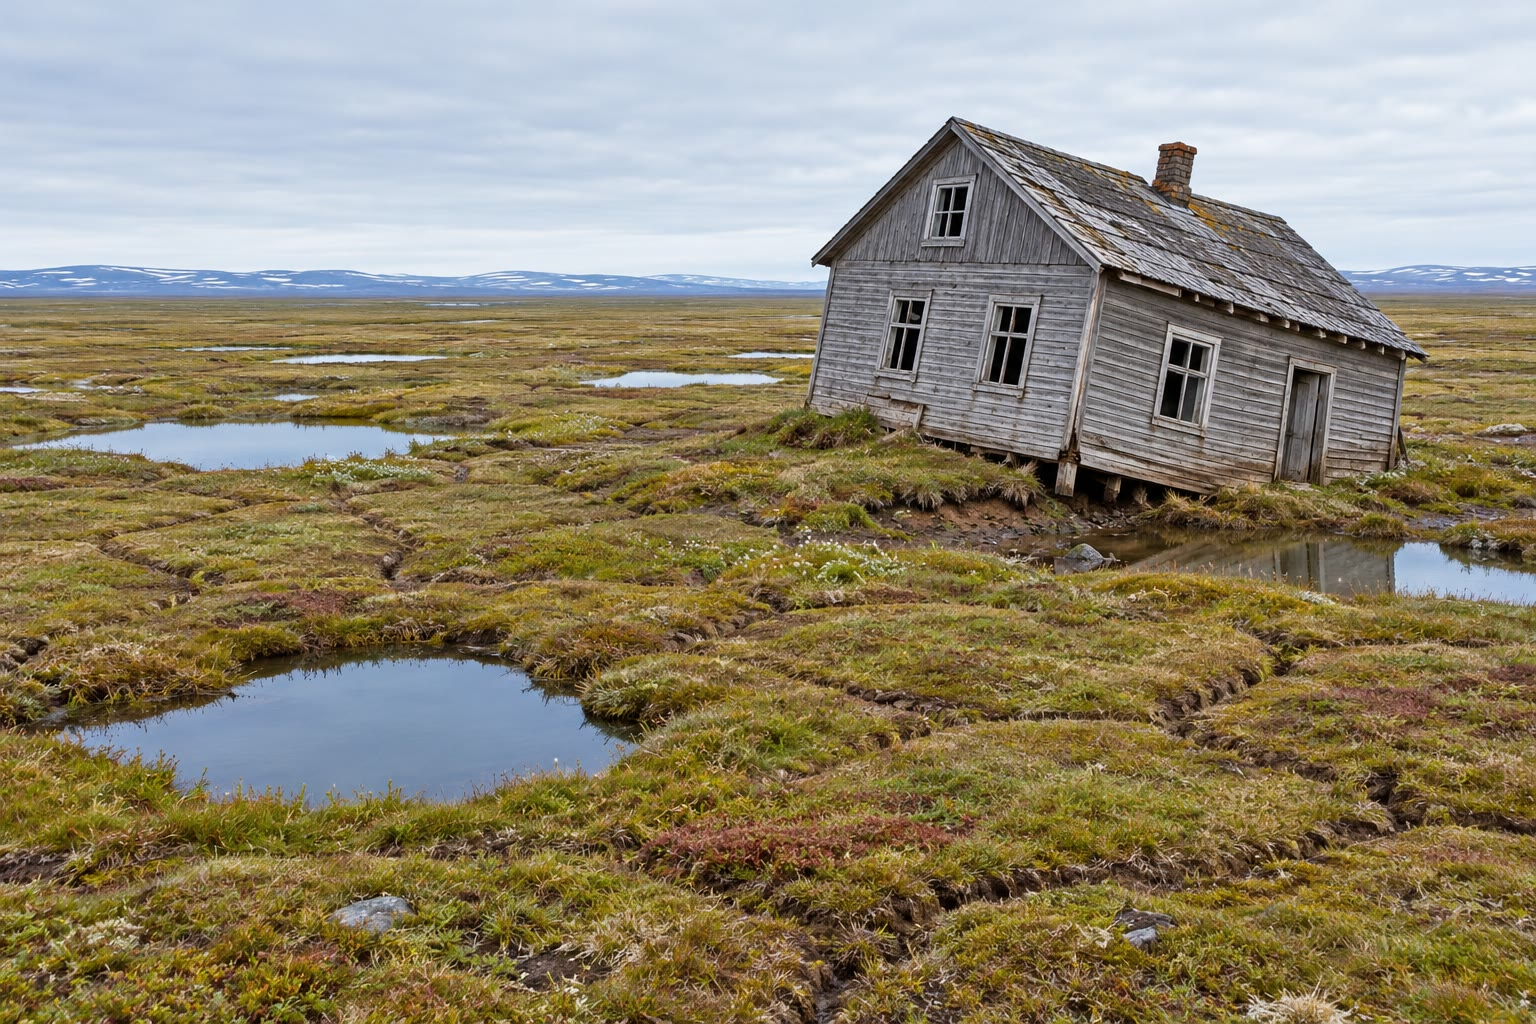
\includegraphics[width=\linewidth]{images/book1/ai/g8-permafrost-house.jpg}
\end{minipage}\hfill
\begin{minipage}[c]{0.46\linewidth}\centering
\begin{tikzpicture}[font=\footnotesize]
  \fill[omLithAlluv] (0,0) rectangle (3.2,-0.6);
  \fill[omIce!70!omLithShale] (0,-0.6) rectangle (3.2,-3.0);
  \foreach \x/\y in {0.4/-1.0, 1.5/-1.3, 2.6/-0.9, 0.9/-1.9, 2.1/-2.2, 0.5/-2.6, 2.8/-2.6}
    \fill[white] (\x,\y) ellipse (0.22 and 0.06);
  \fill[omLithShale!60] (0,-3.0) rectangle (3.2,-3.6);
  \draw[green!45!black, line width=1pt] (0,0) -- (3.2,0);
  \node[anchor=west, align=left] at (3.3,-0.3) {lapisan aktif:\\ mencair setiap\\ musim panas};
  \node[anchor=west, align=left] at (3.3,-1.8) {permafrost:\\ membeku sepanjang\\ tahun, lensa es};
  \node[anchor=west, align=left] at (3.3,-3.3) {tanah yang\\ tidak membeku};
\end{tikzpicture}
\end{minipage}

\smallskip
{\small Kiri: sebuah rumah yang miring di atas \omterm{def:g8:ice-on-earth:permafrost}{permafrost} yang mencair di
tundra (ilustrasi AI dari suatu adegan umum). Kanan: tanah di bawah tundra
(sketsa, tidak berskala).}
\label{fig:g8:ice-on-earth:permafrost}
\end{omfigure}

\section{Zaman es}

Es tidak selalu menutupi bagian Bumi yang sama. Sekitar \num{20000} tahun
yang lalu, \omterm{def:g8:ice-on-earth:ice-sheet}{lapisan es} menutupi sebagian besar Amerika Utara dan Eropa
utara, termasuk Skandinavia. \omterm{def:g8:ice-on-earth:glacier}{Gletser} ketika itu menutupi sekitar
seperempat daratan, dibandingkan dengan sekitar sepersepuluh sekarang.
Begitu banyak air yang terkunci di dalam es ini sehingga \omterm{def:g4:world-physical-map:altitude}{permukaan laut}
lebih dari \qty{120}{m} lebih rendah daripada sekarang: sebagian \omterm{def:g8:the-oceans:seafloor}{paparan
benua} masa kini merupakan daratan kering. Sejak sekitar \num{15000} tahun
yang lalu, \omterm{def:g8:ice-on-earth:ice-sheet}{lapisan es} itu mencair mundur, dan \omterm{def:g4:world-physical-map:altitude}{permukaan laut} naik;
\omterm{def:g4:world-physical-map:altitude}{permukaan laut} mencapai kira-kira \omterm{def:g4:world-physical-map:altitude}{ketinggiannya} yang sekarang sekitar
\num{8000} tahun yang lalu.
% ledger: usgs:lgm, nsidc:ice-sheets, nsidc:ice-cover

\begin{definition}[Zaman es]\label{def:g8:ice-on-earth:ice-age}
Yang disebut \emph{zaman es}\index{zaman es} adalah masa dingin yang
panjang dalam sejarah Bumi, ketika \omterm{def:g8:ice-on-earth:ice-sheet}{lapisan es} meluas jauh melampaui
wilayah kutub dan menutupi sebagian besar \omterm{def:g3:continents-and-oceans:continent}{benua}. Zaman es terakhir
mencapai masa terdinginnya sekitar \num{20000} tahun yang lalu dan
berakhir sekitar \num{12000} tahun yang lalu.
\end{definition}
% ledger: usgs:lgm, nps:u-valley

Jejak \omterm{def:g8:ice-on-earth:ice-age}{zaman es} terakhir ada di mana-mana di daratan yang dahulu
ditutupinya: \omterm{def:g8:ice-on-earth:glacial-landforms}{lembah berbentuk U} yang jauh dari \omterm{def:g8:ice-on-earth:glacier}{gletser} mana pun sekarang,
\omterm{def:g8:ice-on-earth:glacial-landforms}{morena} terminal yang melintangi \omterm{def:g1:landscapes-around-us:landform}{dataran}, bongkah eratik yang tergeletak di
ladang. Dan \omterm{def:g8:ice-on-earth:ice-age}{zaman es} itu bukan satu-satunya. Selama beberapa ratus ribu
tahun terakhir, zaman-zaman es dan masa-masa yang lebih hangat di antaranya
silih berganti berulang kali; kita hidup di salah satu masa yang hangat.
\Cref{ch:g9:climate-past-and-present} menceritakan bagaimana para ilmuwan
membaca kisah panjang ini di dalam es Antarktika sendiri.
% ledger: nps:u-valley, nps:moraines, usgs:erratic

\section{Latihan}

\begin{exercise}[$\star$]\label{exo:g8:ice-on-earth:1}
Dengan memakai penampang memanjang \omterm{def:g8:ice-on-earth:glacier}{gletser} dalam bab ini, sebutkan:
(a) bagian \omterm{def:g8:ice-on-earth:glacier}{gletser} tempat ia bertambah es; (b) bagian tempat ia
kehilangan es; (c) ujung depan \omterm{def:g8:ice-on-earth:glacier}{gletser}; (d) pematang puing \omterm{def:g3:stones-pebbles-sand:rock}{batuan} di
ujungnya.
\end{exercise}

\begin{exercise}[$\star$]\label{exo:g8:ice-on-earth:2}
% ledger: nsidc:firn, nsidc:glacier-flow, nsidc:sea-ice-def
Benar atau salah? Perbaiki kalimat yang salah. (a) \omterm{def:g8:ice-on-earth:glacier}{Gletser} terbuat dari
air \omterm{def:g2:water-on-earth:ocean}{laut} yang membeku. (b) \omterm{def:g4:clouds-rain-snow:precipitation}{Salju} memerlukan sekitar satu tahun untuk
menjadi firn. (c) Ketika \omterm{def:g8:ice-on-earth:glacier}{gletser} menyusut, esnya mengalir mendaki lereng.
(d) \omterm{def:g8:ice-on-earth:sea-ice}{Es laut} di Arktik paling sedikit pada bulan September.
\end{exercise}

\begin{exercise}[$\star$]\label{exo:g8:ice-on-earth:3}
% ledger: usgs:erratic, nsidc:permafrost
Berikan istilah untuk setiap uraian: (a) \omterm{def:g1:landscapes-around-us:landform}{lembah} dengan dasar yang lebar
dan dinding yang curam, yang diukir oleh es; (b) bongkah yang dibawa
\omterm{def:g8:ice-on-earth:glacier}{gletser} jauh dari tempat asalnya; (c) lempeng es terapung yang masih
tersambung dengan es di daratan; (d) tanah yang tetap membeku selama
sekurang-kurangnya dua tahun berturut-turut.
\end{exercise}

\begin{exercise}[$\star$]\label{exo:g8:ice-on-earth:4}
% ledger: nsidc:ice-sheets, nsidc:ice-cover
(a) Dua daratan mana yang sekarang tertutup \omterm{def:g8:ice-on-earth:ice-sheet}{lapisan es}? (b) Mana di antara
keduanya yang akan menaikkan \omterm{def:g4:world-physical-map:altitude}{permukaan laut} lebih tinggi jika seluruh
esnya mencair, dan berapa besarnya? (c) Berapa bagian daratan di Bumi
yang sekarang tertutup es?
\end{exercise}

\begin{exercise}[$\star\star$]\label{exo:g8:ice-on-earth:5}
% ledger: data:b1-nsidc-sea-ice (figdata/grade-8/sea_ice.py)
Gunakan grafik \omterm{def:g8:ice-on-earth:sea-ice}{es laut} Arktik pada bulan September. (a) Bacalah luas
sebarannya pada tahun 1979 dan pada tahun 2012. (b) Berapa juta~km$^2$
luas itu menyusut di antara kedua tahun itu? (c) Berapa bagian dari luas
sebaran tahun 1979 yang telah hilang pada tahun 2012? Bulatkan menjadi
pecahan yang sederhana. (d) Mengapa membandingkan garis tren lebih dapat
diandalkan daripada membandingkan dua tahun saja?
\end{exercise}

\begin{exercise}[$\star\star$]\label{exo:g8:ice-on-earth:6}
% ledger: nsidc:muir, uw:pedersen
Moncong \omterm{def:g8:ice-on-earth:glacier}{Gletser} Muir mundur \qty{12}{km} antara tahun 1941 dan 2004.
(a) Berapa tahun itu? (b) Berapa rata-rata mundurnya per tahun, dalam
meter? Bulatkan sampai puluhan meter terdekat. (c) \omterm{def:g8:ice-on-earth:glacier}{Gletser} Pedersen mundur
\qty{3.2}{km} antara tahun 1984 dan 2021. Berapa rata-rata mundurnya per
tahun? (d) \omterm{def:g8:ice-on-earth:glacier}{Gletser} mana yang menyusut lebih cepat?
\end{exercise}

\begin{exercise}[$\star\star$]\label{exo:g8:ice-on-earth:7}
Jelaskan, dalam beberapa kalimat dan secara berurutan, bagaimana \omterm{def:g4:clouds-rain-snow:precipitation}{salju}
yang turun tinggi di sebuah \omterm{def:g1:landscapes-around-us:landform}{gunung} menjadi es di moncong \omterm{def:g8:ice-on-earth:glacier}{gletser}, jauh di
hilir \omterm{def:g1:landscapes-around-us:landform}{lembah}. Gunakan kata-kata \emph{firn}, \emph{daerah akumulasi},
\emph{mengalir}, dan \emph{daerah ablasi}.
\end{exercise}

\begin{exercise}[$\star\star$]\label{exo:g8:ice-on-earth:8}
% ledger: nsidc:ice-shelves
Dua gelas diisi sampai ketinggian yang sama. Di gelas A, kubus-kubus es
mengapung di atas air; di gelas B, kubus-kubus es yang sama terletak di
atas batu, di luar air. (a) Setelah esnya mencair, di gelas mana
ketinggian airnya naik? (b) Gelas mana yang merupakan model \omterm{def:g8:ice-on-earth:ice-sheet}{gunung es}
yang mencair di \omterm{def:g2:water-on-earth:ocean}{laut}? Dan model \omterm{def:g8:ice-on-earth:ice-sheet}{lapisan es} yang mencair di daratan?
(c) Mengapa pecahnya \omterm{def:g8:ice-on-earth:ice-sheet}{paparan es} tetap penting bagi \omterm{def:g4:world-physical-map:altitude}{ketinggian} \omterm{def:g4:world-physical-map:altitude}{permukaan
laut}?
\end{exercise}

\begin{exercise}[$\star\star$]\label{exo:g8:ice-on-earth:9}
Seorang pejalan kaki menyeberangi \omterm{def:g1:landscapes-around-us:landform}{lembah} lebar yang dasarnya datar dan
dindingnya sangat curam. Di tengah sebuah ladang ia menemukan bongkah
granit sebesar mobil; semua \omterm{def:g3:stones-pebbles-sand:rock}{batuan} di \omterm{def:g1:landscapes-around-us:landform}{lembah} itu adalah batu kapur. Lebih
tinggi lagi, sebuah pematang panjang dari batu-batu yang campur aduk
membentang di sepanjang sisi \omterm{def:g1:landscapes-around-us:landform}{lembah}. (a) Apa bentuk \omterm{def:g1:landscapes-around-us:landform}{lembah} itu, dan apa
yang mengukirnya? (b) Bagaimana bongkah itu sampai di sana? Apa namanya?
(c) Apakah pematang itu, dan apa yang ditunjukkan oleh tingginya di sisi
\omterm{def:g1:landscapes-around-us:landform}{lembah}?
\end{exercise}

\begin{exercise}[$\star\star$]\label{exo:g8:ice-on-earth:10}
% ledger: nsidc:ice-sheets
\omterm{def:g8:ice-on-earth:ice-sheet}{Lapisan es} Antarktika akan menaikkan \omterm{def:g4:world-physical-map:altitude}{permukaan laut} sekitar \qty{58}{m}
jika seluruhnya mencair, dan \omterm{def:g8:ice-on-earth:ice-sheet}{lapisan es} Greenland sekitar \qty{7.4}{m}.
(a) Berapa yang akan ditambahkan oleh sepersepuluh es Greenland? (b) Berapa
yang akan ditambahkan oleh seperseratus es Antarktika? (c) Berapa kali
lebih banyak yang disimpan Antarktika dibandingkan dengan Greenland?
Bulatkan sampai bilangan bulat terdekat.
\end{exercise}

\begin{exercise}[$\star\star\star$]\label{exo:g8:ice-on-earth:11}
% ledger: data:b1-nsidc-sea-ice (figdata/grade-8/sea_ice.py: mean_1980s, mean_2010s, trend)
Rata-rata luas sebaran \omterm{def:g8:ice-on-earth:sea-ice}{es laut} Arktik pada bulan September adalah
\num{7.21}~juta~\unit{km^2} selama tahun 1980--1989 dan
\num{4.65}~juta~\unit{km^2} selama tahun 2010--2019. (a) Satu juta adalah
$10^6$. Tuliskan kedua nilai itu dalam km$^2$, tanpa kata ``juta''.
(b) Berapa besar penurunan rata-rata luas sebaran di antara kedua
dasawarsa itu? (c) Kedua dasawarsa itu berselang 30 tahun. Berapa
penurunannya per dasawarsa? Bandingkan dengan garis tren, yang
\num{0.76}~juta~\unit{km^2} per dasawarsa. (d) Mengapa garis tren yang
lurus tidak dapat diperpanjang selamanya ke masa depan?
\end{exercise}

\begin{exercise}[$\star\star\star$]\label{exo:g8:ice-on-earth:12}
% ledger: usgs:lgm (the shelf slope is exercise data)
Sekitar \num{20000} tahun yang lalu, \omterm{def:g4:world-physical-map:altitude}{permukaan laut} sekitar \qty{120}{m}
lebih rendah daripada sekarang. Di lepas sebuah pantai, \omterm{def:g8:the-oceans:seafloor}{paparan benua}
melandai turun dengan sangat perlahan, \qty{1}{m} untuk setiap
\qty{1}{km} ke arah \omterm{def:g2:water-on-earth:ocean}{laut} (data latihan). (a) Seberapa jauh ke arah \omterm{def:g2:water-on-earth:ocean}{laut}
letak garis pantai pada masa itu? (b) Ke mana perginya air yang
\qty{120}{m} itu? (c) Jelaskan mengapa \omterm{def:g8:ice-on-earth:glacial-landforms}{morena} terminal yang ditemukan
sekarang di sebuah \omterm{def:g1:landscapes-around-us:landform}{dataran}, jauh dari \omterm{def:g4:world-physical-map:range}{pegunungan} mana pun, merupakan
petunjuk tentang \omterm{def:g8:ice-on-earth:ice-age}{zaman es} yang sama.
\end{exercise}

\section{Soal: Mundurnya sebuah gletser yang panjang}

\begin{problem}[{Soal akhir pekan --- ujung depan sebuah gletser gunung
telah diukur setiap sepuluh tahun sejak 1960; kecepatan mundurnya
dihitung, dan lembah yang ditinggalkannya dibaca}]
\label{pb:g8:ice-on-earth:1}
% ledger: nsidc:muir, uw:pedersen, nps:moraines (figdata/grade-8/glacier_retreat.py; Glacier G and its measurements are exercise data)
Setiap sepuluh tahun sejak 1960, sebuah tim mengukur posisi moncong
\omterm{def:g8:ice-on-earth:glacier}{Gletser}~G, sebuah \omterm{def:g8:ice-on-earth:glacier}{gletser} \omterm{def:g1:landscapes-around-us:landform}{lembah} di \omterm{def:g4:world-physical-map:range}{pegunungan}. Jaraknya diukur ke arah
hulu \omterm{def:g1:landscapes-around-us:landform}{lembah} dari sebuah batu penanda~B, yang dicat di dasar \omterm{def:g1:landscapes-around-us:landform}{lembah} di
moncong \omterm{def:g8:ice-on-earth:glacier}{gletser} pada tahun 1960. Sebuah pondok~P berdiri di tepi dasar
\omterm{def:g1:landscapes-around-us:landform}{lembah}, \qty{1980}{m} ke hulu dari~B. \omterm{def:g2:drawing-to-map:map}{Peta} menunjukkan moncong pada setiap
pengukuran dan pematang tepat di bawah moncong tahun 1960.

\begin{center}
\begin{tikzpicture}
\begin{axis}[axis equal image, width=12.5cm, xmin=-500, xmax=2600, ymin=-760, ymax=760,
  axis lines=none, clip=true]
  \fill[black!13] (axis cs:-500,-760) rectangle (axis cs:2600,760);
  \addplot[fill=white, draw=none] table[x=y, y=x] {figdata/out/grade-8-glacier_retreat-floor.dat} -- cycle;
  \addplot[fill=omIce, draw=none] table[x=y, y=x] {figdata/out/grade-8-glacier_retreat-ice.dat} -- cycle;
  \addplot[black!70, line width=0.8pt] table[x=y, y=x] {figdata/out/grade-8-glacier_retreat-walls.dat};
  \addplot[omCold, line width=0.9pt] table[x=y, y=x] {figdata/out/grade-8-glacier_retreat-fronts.dat};
  \addplot[omLithCongl!80!black, line width=3pt] table[x=y, y=x] {figdata/out/grade-8-glacier_retreat-moraine.dat};
  \addplot[only marks, mark=none, nodes near coords, point meta=explicit symbolic,
    every node near coord/.style={anchor=south, rotate=90, font=\scriptsize, inner sep=1pt}]
    table[x=y, y=x, meta=year] {figdata/out/grade-8-glacier_retreat-labels.dat};
  \addplot[only marks, mark=*, mark size=2pt] coordinates {(0,0)};
  \node[font=\footnotesize\bfseries, anchor=south east] at (axis cs:-10,10) {B};
  \addplot[only marks, mark=square*, mark size=2.6pt, omDef] coordinates {(1980,-560)};
  \node[font=\footnotesize\bfseries, anchor=north] at (axis cs:1980,-590) {P};
  \node[font=\scriptsize, anchor=west] at (axis cs:-480,-590) {ke hulu lembah $\longrightarrow$};
  \node[font=\scriptsize] at (axis cs:2250,0) {es pada 2020};
  \draw[black, line width=1.2pt] (axis cs:2000,640) -- (axis cs:2500,640)
    node[midway, below, font=\scriptsize] {\qty{500}{m}};
\end{axis}
\end{tikzpicture}

\smallskip
{\small
\begin{tabular}{|l|c|c|c|c|c|c|c|}
\hline
tahun & 1960 & 1970 & 1980 & 1990 & 2000 & 2010 & 2020 \\
\hline
jarak moncong dari B (m) & 0 & 180 & 330 & 520 & 700 & 880 & 1080 \\
\hline
\end{tabular}}
\end{center}

\noindent\textbf{Bagian I --- Posisi-posisi moncong.}\par\nopagebreak
\begin{enumerate}[beginpenalty=10000]
  \item Seberapa jauh moncong itu mundur antara tahun 1960 dan 2020?
  \item Hitunglah seberapa jauh moncong itu mundur pada setiap dasawarsa.
        Pada dasawarsa mana mundurnya paling sedikit? Paling banyak?
  \item Apakah \omterm{def:g8:ice-on-earth:glacier}{gletser} itu sudah berhenti mengalir menuruni lereng?
        Jelaskan.
  \item Pematang gelap tepat di bawah moncong tahun 1960 terbuat dari puing
        \omterm{def:g3:stones-pebbles-sand:rock}{batuan} yang campur aduk. Apa namanya, dan bagaimana terbentuknya?
\end{enumerate}

\noindent\textbf{Bagian II --- Kecepatan mundurnya.}\par\nopagebreak
\begin{enumerate}[resume, beginpenalty=10000]
  \item Berapa rata-rata mundurnya per dasawarsa antara tahun 1960 dan
        2020?
  \item Dan per tahun?
  \item \omterm{def:g8:ice-on-earth:glacier}{Gletser} Muir mundur \qty{12}{km} dalam 63 tahun, sekitar
        \qty{190}{m} setahun. Berapa kali lebih cepat itu dibandingkan
        dengan \omterm{def:g8:ice-on-earth:glacier}{Gletser}~G?
  \item Apakah \omterm{def:g8:ice-on-earth:glacier}{Gletser}~G memperoleh lebih banyak es di daerah akumulasinya
        daripada yang hilang di daerah ablasinya, atau lebih sedikit?
        Jelaskan.
\end{enumerate}

\noindent\textbf{Bagian III --- Lembah yang ditinggalkannya.}\par\nopagebreak
\begin{enumerate}[resume, beginpenalty=10000]
  \item Bentuk apa yang kamu perkirakan dimiliki dasar \omterm{def:g1:landscapes-around-us:landform}{lembah} di antara B
        dan moncong tahun 2020 dalam penampang melintang? Mengapa?
  \item Pada tahun 2020, seberapa jauh moncong itu dari titik yang sejajar
        dengan pondok?
  \item Dengan kecepatan rata-rata dari Bagian~II, berapa tahun yang
        diperlukan moncong itu untuk mencapai titik yang sejajar dengan
        pondok? Pada tahun berapa hal itu terjadi?
  \item Berikan satu alasan mengapa tahun ini bukan sebuah prakiraan.
\end{enumerate}
\end{problem}
